\documentclass[12pt]{report}
\usepackage[utf8]{inputenc}
\usepackage[russian]{babel}
%\usepackage[14pt]{extsizes}
\usepackage{listings}
\usepackage{graphicx}
\usepackage{amsmath,amsfonts,amssymb,amsthm,mathtools} 
\usepackage{pgfplots}
\usepackage{filecontents}
\usepackage{indentfirst}
\usepackage{eucal}
\usepackage{amsmath}
\usepackage{enumitem}
\frenchspacing

\usepackage{indentfirst} % Красная строка


%\usetikzlibrary{datavisualization}
%\usetikzlibrary{datavisualization.formats.functions}

\usepackage{amsmath}




% Для листинга кода:
\lstset{ %
language=haskell,                 % выбор языка для подсветки (здесь это С)
basicstyle=\small\sffamily, % размер и начертание шрифта для подсветки кода
numbers=left,               % где поставить нумерацию строк (слева\справа)
numberstyle=\tiny,           % размер шрифта для номеров строк
stepnumber=1,                   % размер шага между двумя номерами строк
numbersep=5pt,                % как далеко отстоят номера строк от подсвечиваемого кода
showspaces=false,            % показывать или нет пробелы специальными отступами
showstringspaces=false,      % показывать или нет пробелы в строках
showtabs=false,             % показывать или нет табуляцию в строках
frame=single,              % рисовать рамку вокруг кода
tabsize=2,                 % размер табуляции по умолчанию равен 2 пробелам
captionpos=t,              % позиция заголовка вверху [t] или внизу [b] 
breaklines=true,           % автоматически переносить строки (да\нет)
breakatwhitespace=false, % переносить строки только если есть пробел
escapeinside={\#*}{*)}   % если нужно добавить комментарии в коде
}

\usepackage[left=2cm,right=2cm, top=2cm,bottom=2cm,bindingoffset=0cm]{geometry}
% Для измененных титулов глав:
\usepackage{titlesec, blindtext, color} % подключаем нужные пакеты
\definecolor{gray75}{gray}{0.75} % определяем цвет
\newcommand{\hsp}{\hspace{20pt}} % длина линии в 20pt
% titleformat определяет стиль
\titleformat{\chapter}[hang]{\Huge\bfseries}{\thechapter\hsp\textcolor{gray75}{|}\hsp}{0pt}{\Huge\bfseries}


% plot
\usepackage{pgfplots}
\usepackage{filecontents}
\usetikzlibrary{datavisualization}
\usetikzlibrary{datavisualization.formats.functions}
\RequirePackage[
  style=gost-numeric,
  language=auto,
  autolang=other,
  sorting=none,
]{biblatex}

\addbibresource{bib.bib}
\begin{document}
%\def\chaptername{} % убирает "Глава"
\thispagestyle{empty}
\begin{titlepage}
	\noindent \begin{minipage}{0.15\textwidth}
	
\includegraphics[width=\linewidth]{b_logo}
	\end{minipage}
	\noindent\begin{minipage}{0.9\textwidth}\centering
		\textbf{Министерство науки и высшего образования Российской Федерации}\\
		\textbf{Федеральное государственное бюджетное образовательное учреждение высшего образования}\\
		\textbf{~~~«Московский государственный технический университет имени Н.Э.~Баумана}\\
		\textbf{(национальный исследовательский университет)»}\\
		\textbf{(МГТУ им. Н.Э.~Баумана)}
	\end{minipage}
	
	\noindent\rule{18cm}{3pt}
	\newline\newline
	\noindent ФАКУЛЬТЕТ $\underline{\text{«Информатика и системы управления»}}$ \newline\newline
	\noindent КАФЕДРА $\underline{\text{«Программное обеспечение ЭВМ и информационные технологии»}}$\newline\newline\newline\newline\newline
	
	
	\begin{center}
		\noindent\begin{minipage}{1.3\textwidth}\centering
			\Large\textbf{  Отчёт по лабораторной работе №6 по дисциплине}\newline
			\textbf{ "Методы машинного обучения"}\newline\newline
		\end{minipage}
	\end{center}
	
	\noindent\textbf{Тема} $\underline{\text{Классификатор на базе многослойного персептрона}}$\newline\newline
	\noindent\textbf{Студент} $\underline{\text{Варламова Е. А.}}$\newline\newline
	\noindent\textbf{Группа} $\underline{\text{ИУ7-23М}}$\newline\newline
	\noindent\textbf{Оценка (баллы)} $\underline{\text{~~~~~~~~~~~~~~~~~~~~~~~~~~~}}$\newline\newline
	\noindent\textbf{Преподаватели} $\underline{\text{Солодовников Владимир Игоревич}}$\newline\newline\newline
	
	\begin{center}
		\vfill
		Москва~---~\the\year
		~г.
	\end{center}
\end{titlepage}
\large
\setcounter{page}{2}
\def\contentsname{СОДЕРЖАНИЕ}
\renewcommand{\contentsname}{СОДЕРЖАНИЕ}
\tableofcontents
\renewcommand\labelitemi{---}
\newpage
\chapter{Теоретическая часть}

Многослойный персептрон -- это тип нейронной сети, состоящей из нескольких слоев нейронов, которые взаимодействуют друг с другом. Он является одним из наиболее распространенных видов искусственных нейронных сетей и широко применяется в области машинного обучения и глубокого обучения. Многослойный персептрон состоит из входного слоя, скрытых слоев и выходного слоя, причем каждый слой содержит нейроны, которые передают сигналы друг другу и выполняют сложные вычисления. Благодаря способности обучаться на основе данных и корректировать свои веса, многослойный персептрон способен решать разнообразные задачи, такие как классификация, регрессия и распознавание образов.

Целью данной лабораторной работы является применение многослойного персептрона для решения задачи классификации областей признакового пространства.
Для этого необходимо решить следующие задачи:
\begin{itemize}
    \item формализовать задачу;
    \item описать алгоритм работы многослойного персептрона;
    \item привести особенности реализации ПО, решающего поставленную задачу;
    \item оценить точность, полноту, F-меру классификатора; построить матрицу ошибок; построить графики изменения среднеквадратических ошибок на обучающей и тестовой  выборках.
    \item провести исследование работы нейросети в зависимости от выбранной функции активации.
\end{itemize}

\section{Постановка задачи}

Осуществить генерацию исходных данных, которые представляют собой двумерное признаковое пространство, сгруппированное в 6 или более областей, отнесенных не менее чем к 4 классам. В каждой области содержится не менее 50 примеров, и данные распределены по нормальному закону распределения.  

В ходе выполнения работы:
\begin{enumerate}
    \item Визуализировать сгенерированные данные на плоскости.
    \item Для  сгенерированного датасета осуществить построение классификатор на базе многослойного персептрона. 
    \item Обосновать выбор числа слоев и нейронов в каждом слое. 
    \item Сравнить работу нейросети в зависимости от выбранной функции активации (сигмоида с разными значениями параметра, определяющего крутизну (b=1,b=100), ReLU).
    \item В процессе обучения визуализировать разделяющие поверхности промежуточного слоя. 
    \item В процессе обучения построить графики изменения среднеквадратических ошибок на обучающей и тестовой  выборках. Обосновать момент остановки процесса обучения.
	Оценить точность, полноту, F-меру. Построить матрицу ошибок.
    \item Предусмотреть дополнительную возможность ввода пользователем новых, не входящих в сгенерированный датасет данных. Визуализировать их совместно с обучающей выборкой и разделяющими поверхностями, осуществить их классификацию. 
\end{enumerate}
\section{Основные понятия нейронной сети}
Перечислим основные понятия, используемые в нейросетях.
\begin{itemize}
    \item Нейрон (или узел): Нейрон -- это базовый элемент нейронной сети, имитирующий функцию биологического нейрона. 
    Он принимает входные сигналы, обрабатывает их и генерирует выходной сигнал. 
    Каждый нейрон обычно имеет несколько входов, каждый из которых соответствует весу (степени важности) исходного сигнала.
    \item Веса: Веса представляют собой параметры, которые определяют степень важности входной информации для каждого нейрона.
    Они отражают силу связей между нейронами и являются ключевыми для эффективного обучения нейронной сети.
    \item Функция активации: Функция активации определяет выходное значение нейрона на основе его взвешенного входа и возможно добавления смещения. 
    Различные функции активации, такие как ReLU, сигмоида, tanh, используются для введения нелинейности в нейронные сети.
    \item Структура и связи:  Нейронные сети могут быть организованы в различные архитектуры, такие как многослойные перцептроны, сверточные нейронные сети, рекуррентные нейронные сети и другие. 
    Связи между нейронами формируют слои и определяют поток информации в сети.
    \item Функция потерь: Функция потерь измеряет разницу между предсказанными значениями модели и фактическими значениями. 
    Во время обучения нейронная сеть минимизирует эту функцию, чтобы улучшить качество своих прогнозов.
    \item Оптимизатор: Оптимизатор используется для коррекции весов нейронов в ходе обучения, с целью минимизации функции потерь.
    Примером может служить алгоритм градиентного спуска.
    \item Слои: Нейронные сети состоят из различных слоев, таких как входной, скрытый и выходной слои. 
    Каждый слой выполняет определенные вычисления и обработку данных.
    \item Обучающие данные и цели: Нейронные сети обучаются на основе обучающих данных и их соответствующих целей (или меток). 
    Эти данные используются для корректировки весов нейронов в процессе обучения.
\end{itemize}

\section{Обучение нейросети}

Обучение нейросети состоит из нескольких эпох (итераций). В течение одной эпохи обучения нейронной сети происходит несколько этапов, которые повторяются для каждого обучающего примера:
\begin{enumerate}
    \item прямое распространение:
    \begin{itemize}
        \item входные данные подаются на входной слой нейронов;
        \item данные передаются через скрытые слои, взвешиваются с использованием соответствующих весов и агрегируются;
        \item агрегированные значения проходят через функции активации каждого нейрона в скрытых слоях и выходном слое, что приводит к формированию выходов сети;
    \end{itemize}
    \item  оценка ошибки : вычисляется ошибка между выходами сети и ожидаемыми значениями (целевыми метками/метками классов);
    \item обратное распространение ошибки:
    \begin{itemize}
        \item ошибка распространяется обратно через сеть, начиная с последнего слоя и двигаясь к входному слою;
        \item для каждого слоя вычисляется градиент функции потерь по весам и смещениям сети;
    \end{itemize}
    \item обновление весов, чтобы уменьшить ошибку модели: используя градиент ошибки, веса сети обновляются с использованием метода оптимизации, такого как стохастический градиентный спуск или его модификации;
\end{enumerate}

Эти этапы повторяются для каждой эпохи обучения с тем, чтобы постепенно корректировать веса сети и уменьшать ошибку прогноза. Процесс обучения заключается в том, чтобы минимизировать ошибку модели и достичь желаемой производительности в решении конкретной задачи.

\section{Функция активации ReLU}
Функция ReLU -- это популярная функция активации в нейронных сетях, которая обладает нелинейными свойствами. 
Ее формула определяется следующим образом:
\begin{equation}
    f(x) = \max(\alpha * x, x) 
\end{equation}

Таким образом, ReLU функция активации принимает следующие значения:
\begin{equation}
    f(x) = \begin{cases} 
    x, & \mbox{if } x > 0 \\ 
    \alpha * x, & \mbox{if } x \leq 0 
    \end{cases} 
\end{equation}

ReLU функция  подходит для использования в нейронных сетях по нескольким причинам, включая то, что она обеспечивает нелинейность (что важно для изучения сложных функций) и простоту вычисления.

\section{Сигмоидная функция активации}
Сигмоидная функция активации используется для преобразования взвешенной суммы входов нейрона в диапазоне от 0 до 1. Это позволяет моделировать нелинейные зависимости и обеспечивает гладкое изменение выхода нейрона.

Формула сигмоидной функции активации выглядит следующим образом:
\begin{equation}
     \sigma(x) = \frac{1}{1 + e^{-\alpha x}}
\end{equation}
   
где 
\begin{itemize}
    \item $x$ -- входное значение нейрона
    \item $\sigma(x)$ -- выходное значение после применения функции активации
    \item $\alpha$ -- параметр функции активации.
\end{itemize}

Сигмоидная функция активации широко используется в задачах классификации, так как ее выход можно интерпретировать как вероятность принадлежности к определенному классу. Однако, она имеет недостатки, такие как проблема затухания градиента при обратном распространении ошибки. В связи с этим, сегодня более популярными являются другие функции активации, такие как ReLU и их модификации.

\chapter{Практическая часть}

\section{Выбор средств разработки}
В качестве языка программирования был использован язык Python, поскольку этот язык кроссплатформенный и для него разработано огромное количество библиотек и модулей, решающих разнообразные задачи. 

В частности, имеются библиотеки, включающие в себя алгоритм многослойного персептрона в библиотеке \cite{bib:scipy}.

\section{Исследование ПО}

В листинге \ref{lst:gen1} представлен код классификации.

\begin{lstlisting}[label=lst:gen1,caption=Код классификации]
import numpy as np
import matplotlib.pyplot as plt
from sklearn.datasets import make_blobs
import imageio
import tensorflow as tf
from sklearn.model_selection import train_test_split
from sklearn.metrics import accuracy_score, precision_score, recall_score, f1_score, confusion_matrix
import seaborn as sns
from sklearn.metrics import mean_squared_error
from tensorflow.keras import utils
import pandas as pd
EPOCHS_COUNT = 50
def draw_line(
        x_data: np.ndarray,
        w_1: float,
        w_2: float,
        w_c: float):
    y_arr = -(w_1 * x_data + w_c) / w_2
    plt.plot(x_data, y_arr, linestyle='-')
    return 
def show_lines(x_min: float, x_max: float, neurons: np.ndarray, bias: np.ndarray):
    line_data_x = np.arange(x_min, x_max, (x_min + x_max) / 4)
    # w_1*x + w_2*y + w_c = 0
    # y = -(w_1*x + w_c) / w_2
    for w_1, w_2, w_c in zip(neurons[0], neurons[1], bias):
        draw_line(line_data_x, w_1, w_2, w_c)
    return 
def gen_data():
    n_samples = 300
    n_features = 2
    n_classes = 4
    X, y = make_blobs(n_samples=[300, 250, 200, 150], n_features=n_features, centers=None, cluster_std=1, random_state=42)
    X_additional, y_additional = make_blobs(n_samples=[150, 300], n_features=n_features, centers=None, cluster_std=1, random_state=45)
    X = np.vstack([X, X_additional])
    y = np.hstack([y, y_additional])
    return X, y
def draw_data(X, y):
    plt.figure(figsize=(8, 6))
    plt.scatter(X[:, 0], X[:, 1], c=y, cmap='viridis', edgecolors='k')
    plt.title('Сгенерированные данные')
    plt.xlabel('Признак 1')
    plt.ylabel('Признак 2')
    plt.savefig("data_viz.png")
    
def custom_activation(alpha=1.0):
    def activation(x):
        return 1 / (1 + tf.exp(-alpha * x))
    return activation
def plot_layer(model, X, y, name_graph):
    x_min, x_max = X[:, 0].min() - 1, X[:, 0].max() + 1
    y_min, y_max = X[:, 1].min() - 1, X[:, 1].max() + 1
    xx, yy = np.meshgrid(np.arange(x_min, x_max, 0.1), np.arange(y_min, y_max, 0.1))
    grid_points = np.c_[xx.ravel(), yy.ravel()]
    
    Z = model.predict(grid_points)
    Z = np.argmax(Z, axis=1).reshape(xx.shape)

    plt.figure(figsize=(8, 6))
    plt.contourf(xx, yy, Z, alpha=0.8)
    plt.scatter(X[:, 0], X[:, 1], c=y, cmap='viridis', edgecolors='k')
    plt.title('Разделяющие поверхности промежуточного слоя')
    plt.xlabel('Признак 1')
    plt.ylabel('Признак 2')
    plt.xlim(xx.min(), xx.max())
    plt.ylim(yy.min(), yy.max())
    show_lines(x_min, x_max, model.layers[0].get_weights()[0], model.layers[0].get_weights()[1])

    plt.savefig(name_graph)
    plt.clf()
    
X, y = gen_data()

draw_data(X, y)

X_train, X_test, y_train, y_test = train_test_split(X, y, test_size=0.2, random_state=42)
model_names = ['relu_1', "relu_100", "sigmoid_1", "sigmoid_5"]

models = [
    tf.keras.models.Sequential([
        tf.keras.layers.Dense(6, activation=tf.keras.layers.LeakyReLU(alpha=1), input_dim=2),
        tf.keras.layers.Dense(4, activation='softmax')]), #]#,#]#,
    tf.keras.models.Sequential([
        tf.keras.layers.Dense(6, activation=tf.keras.layers.LeakyReLU(alpha=100), input_dim=2),
        tf.keras.layers.Dense(4, activation='softmax')]),
    tf.keras.models.Sequential([
        tf.keras.layers.Dense(6, activation=custom_activation(alpha=1.0), input_dim=2),
        tf.keras.layers.Dense(4, activation='softmax')]),
    tf.keras.models.Sequential([
        tf.keras.layers.Dense(6, activation=custom_activation(alpha=5), input_dim=2),
        tf.keras.layers.Dense(4, activation='softmax')])    ]
model_num = 0
for model in models:
    model.compile(optimizer='adam', loss='sparse_categorical_crossentropy', metrics=['accuracy'])
    name = model_names[model_num]
    epochs_ctr = 0

    images = []
    errs_train = []
    errs_test = []
    layers = np.arange(1, EPOCHS_COUNT + 1)
    def plot_intermediate_layer(model, X):
        global epochs_ctr
        epochs_ctr += 1
        plot_layer(model, X, y_test, f"img_{name}_{epochs_ctr}.png")
        y_train_pred = model.predict(X_train)
        y_train_pred = np.argmax(y_train_pred, axis=1)
        y_test_pred = model.predict(X_test)
        y_test_pred = np.argmax(y_test_pred, axis=1)
        errs_train.append(mean_squared_error(y_train, y_train_pred))
        errs_test.append(mean_squared_error(y_test, y_test_pred))

    history = model.fit(X_train, y_train, batch_size=5, epochs=EPOCHS_COUNT, validation_data=(X_test, y_test), callbacks=[tf.keras.callbacks.LambdaCallback(on_epoch_end=lambda epoch, logs: plot_intermediate_layer(model, X_test))])

    plt.plot(layers, errs_train, label='Обучающая выборка')
    plt.plot(layers, errs_test, label='Контрольная выборка')
    plt.legend()
    plt.title('СКО')
    plt.savefig(f"std_{name}.png")
    plt.clf()
    
    for i in range(1, EPOCHS_COUNT+1):
        images.append(imageio.imread(f"img_{name}_{i}.png"))
    imageio.mimsave(f'{name}_training_history.gif', images, duration=1000)

    y_pred = model.predict(X_test)
    y_pred = np.argmax(y_pred, axis=1)

    accuracy = accuracy_score(y_test, y_pred)
    precision = precision_score(y_test, y_pred, average='weighted')
    recall = recall_score(y_test, y_pred, average='weighted')
    f1 = f1_score(y_test, y_pred, average='weighted')
    conf_matrix = confusion_matrix(y_test, y_pred)

    sns.heatmap(conf_matrix, annot=True)
    plt.title(f'acc={accuracy:.2f}, prec={precision:.2f}, Recall={recall:.2f}, f1={f1:.2f}')

    plt.savefig(f"matrix_errors_{name}.png")
    plt.clf()
    model_num += 1

    plot_layer(model, X_test, y_test, f"before_{name}.png")
    want = "0"
    u = 0
    while want == "1":
        print("Хотите ввести точку? (1 -- да)")
        want = input()
        if want == "1":
            x1 = float(input("x1: "))
            x2 = float(input("x2: "))
            cluster = int(input("cluster: (0, 1, 2, 3): "))
            
            
            plot_layer(model, np.vstack([X_test, [x1, x2]]), np.append(y_test, cluster), f"after_{name}_{u}.png")
            u += 1
\end{lstlisting}

Были сгенерированы входные данные, показанные на рисунке \ref{fig:data}.

\begin{figure}[h!]
  \centering
  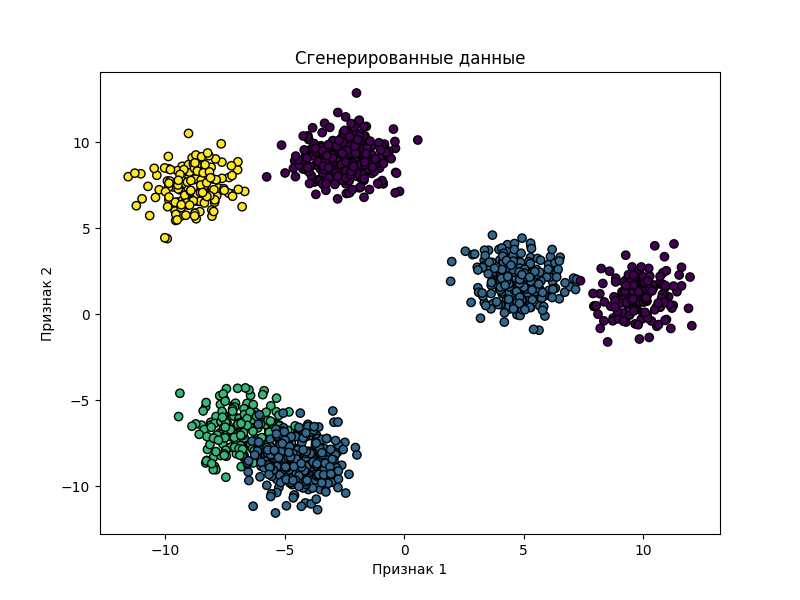
\includegraphics[width = \linewidth]{data_viz.png}
  \caption{Входные данные}
  \label{fig:data}
\end{figure}

Были использованы 4 функции активации для обучения 4 классификаторов на основе многослойного персептрона:
\begin{enumerate}
    \item ReLU со значением $\alpha = 1$;
    \item ReLU со значением $\alpha = 100$;
    \item сигмоидная со значением $\alpha = 1$;
    \item сигмоидная со значением $\alpha = 5$.
\end{enumerate}

Для каждого классификатора было необходимо оценить точность, полноту, F-меру классификатора; построить матрицу ошибок; построить графики изменения среднеквадратических ошибок на обучающей и тестовой  выборках. Соответствующие значения приведены на рисунках \ref{fig:relu_1_matrix}-\ref{fig:sigmoid_5_std}.
\newpage
\begin{figure}[h!]
  \centering
  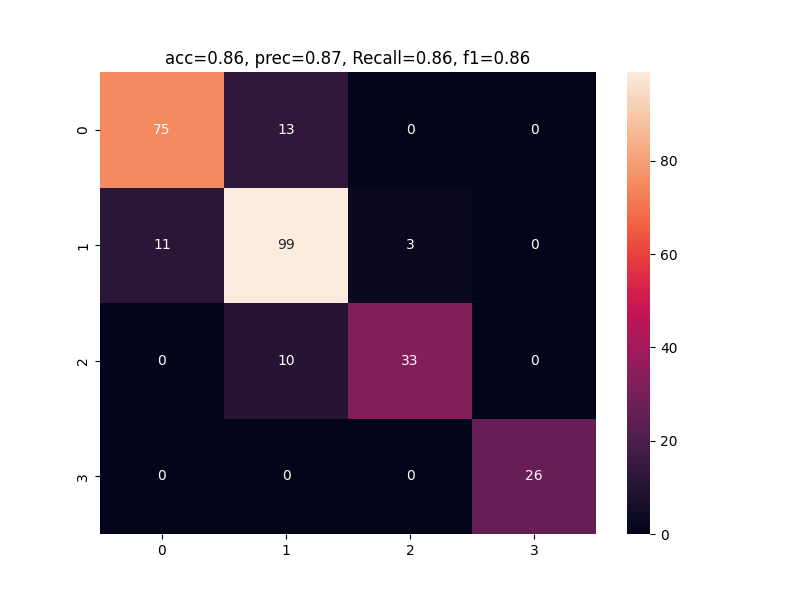
\includegraphics[width = \linewidth / 2]{matrix_errors_relu_1.png}
  \caption{матрица ошибок и оценки точности для ReLU, alpha = 1}
  \label{fig:relu_1_matrix}
\end{figure}

\begin{figure}[h!]
  \centering
  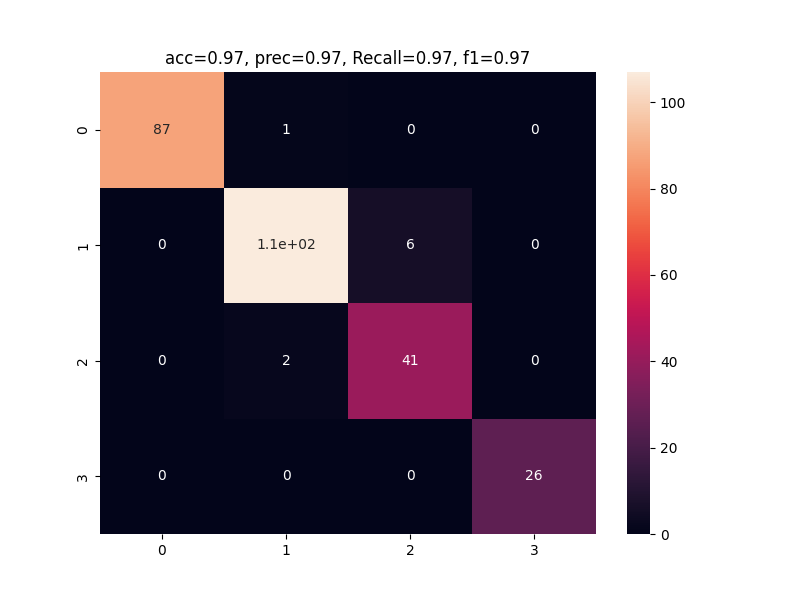
\includegraphics[width = \linewidth / 2]{matrix_errors_relu_100.png}
  \caption{матрица ошибок и оценки точности для ReLU, alpha = 100}
  \label{fig:relu_100_matrix}
\end{figure}
\newpage
\begin{figure}[h!]
  \centering
  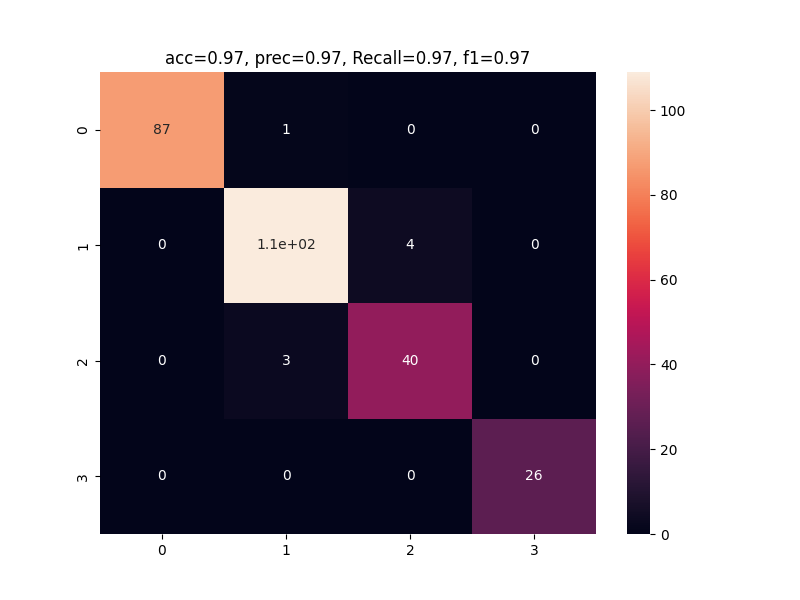
\includegraphics[width = \linewidth / 2]{matrix_errors_sigmoid_1.png}
  \caption{матрица ошибок и оценки точности для сигмоидной, alpha = 1}
  \label{fig:sigmoid_1_matrix}
\end{figure}

\begin{figure}[h!]
  \centering
  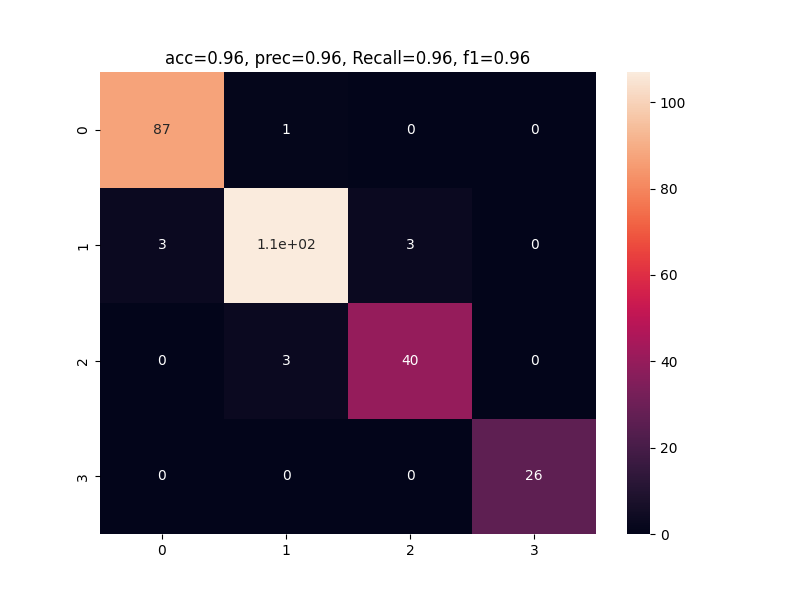
\includegraphics[width = \linewidth / 2]{matrix_errors_sigmoid_5.png}
  \caption{матрица ошибок и оценки точности для сигмоидной, alpha = 5}
  \label{fig:sigmoid_5_matrix}
\end{figure}

\begin{figure}[h!]
  \centering
  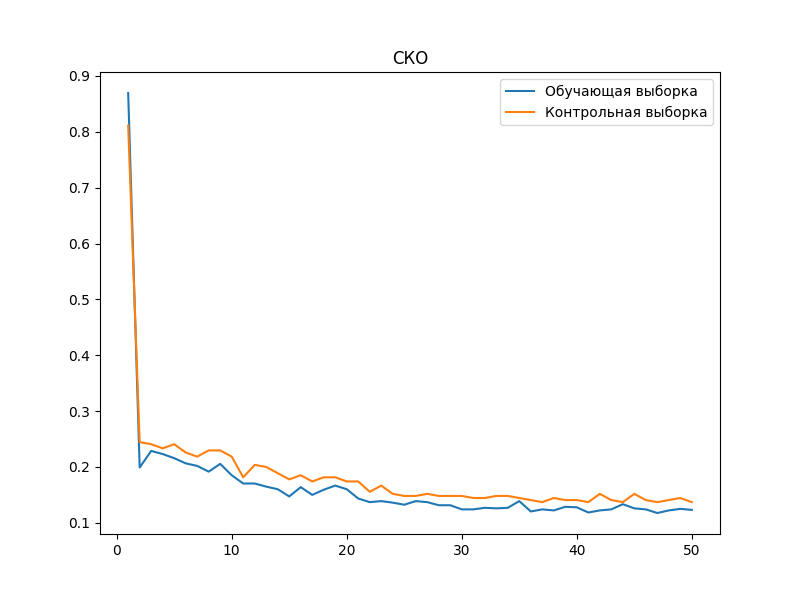
\includegraphics[width = \linewidth / 2]{std_relu_1.png}
  \caption{среднеквадратические ошибки для ReLU, alpha = 1}
  \label{fig:relu_1_std}
\end{figure}
\newpage
\begin{figure}[h!]
  \centering
  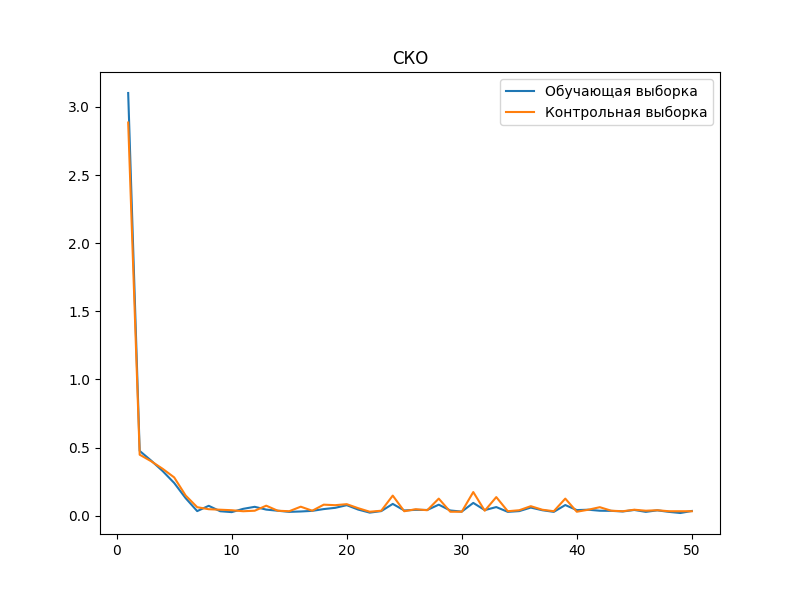
\includegraphics[width = \linewidth / 2]{std_relu_100.png}
  \caption{среднеквадратические ошибки для ReLU, alpha = 100}
  \label{fig:relu_100_std}
\end{figure}

\begin{figure}[h!]
  \centering
  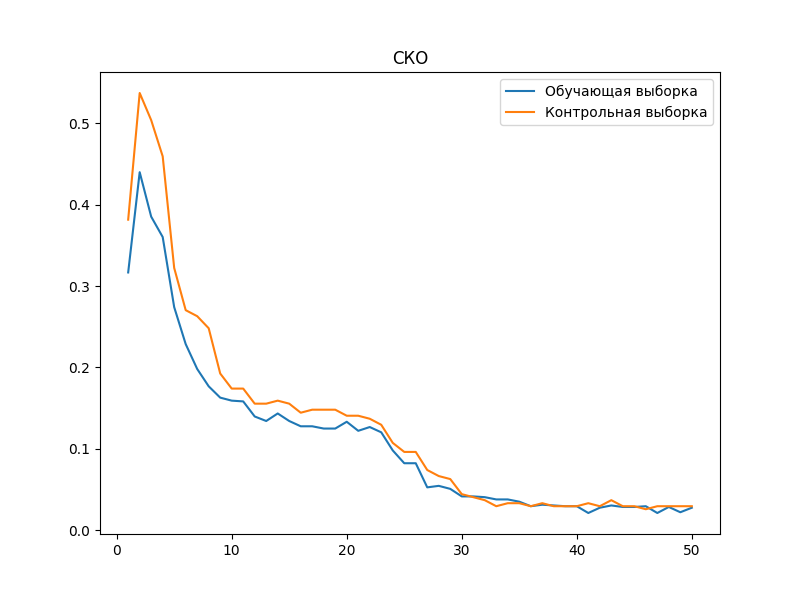
\includegraphics[width = \linewidth / 2]{std_sigmoid_1.png}
  \caption{среднеквадратические ошибки для сигмоидной, alpha = 1}
  \label{fig:sigmoid_1_std}
\end{figure}

\begin{figure}[h!]
  \centering
  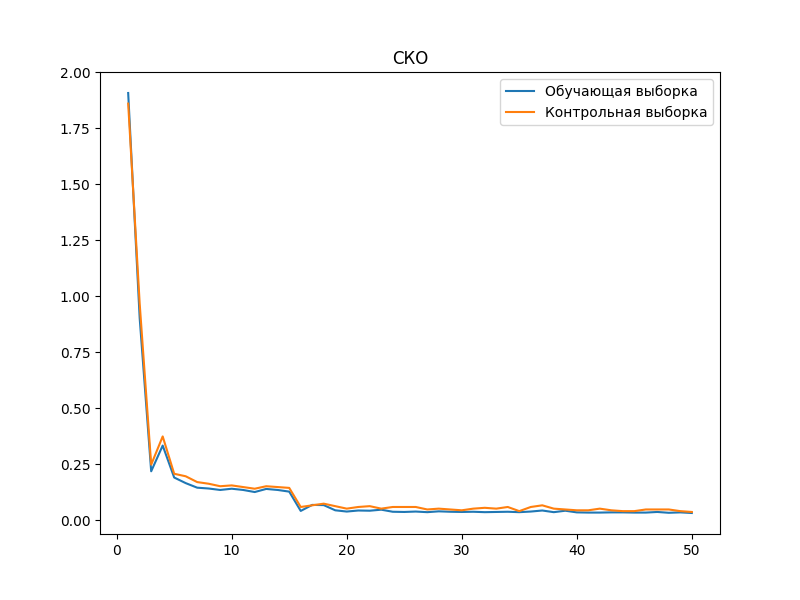
\includegraphics[width = \linewidth / 2]{std_sigmoid_5.png}
  \caption{среднеквадратические ошибки для сигмоидной, alpha = 5}
  \label{fig:sigmoid_5_std}
\end{figure}

\newpage

Для обучения классифкатора был выбран один промежуточный слой нейронов и 6 нейронов в нем. Определение оптимального числа нейронов было осуществлено из геометрических соображений после оценки сгенерированных данных. 

Правильность выбора 6 нейронов промежуточного слоя может быть проилюстрирована следующим образом. Построим прямые с помощью весов и смещений промежуточного слоя. 

На рисунках \ref{fig:div1}-\ref{fig:div5} видим, что прямые проходят по границам областей на моделях с сигмоидной функцией активации.

\begin{figure}[h!]
  \centering
  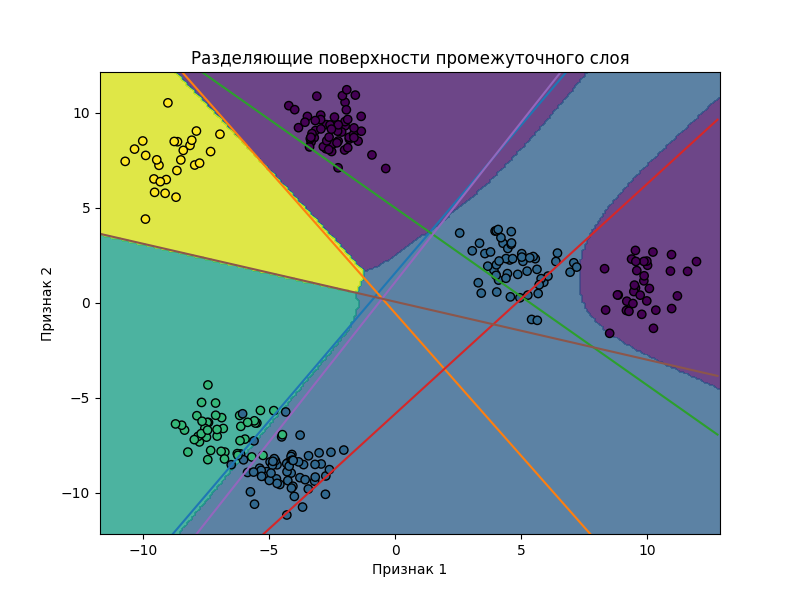
\includegraphics[width = \linewidth / 2]{img_sigmoid_1_50.png}
  \caption{разделяющие поверхности промежуточного слоя для сигмоидной, alpha = 1}
  \label{fig:div1}
\end{figure}
\newpage

\begin{figure}[h!]
  \centering
  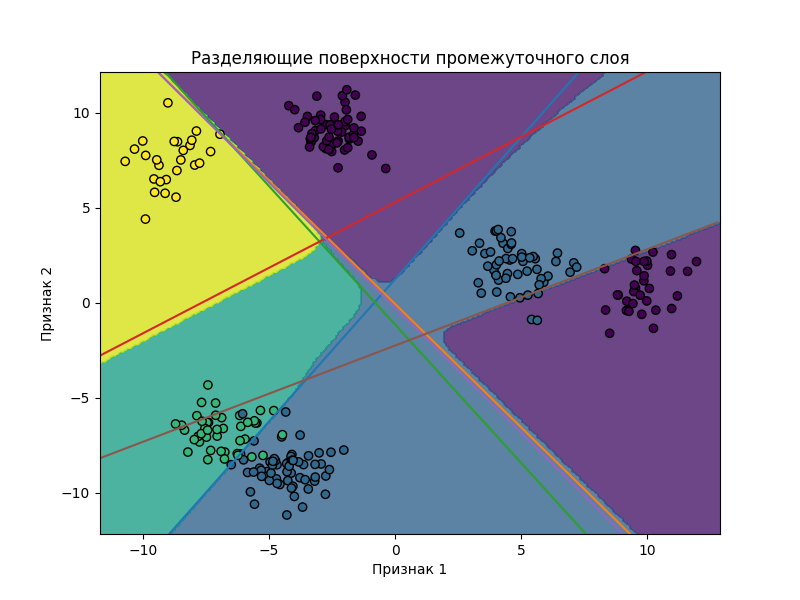
\includegraphics[width = \linewidth / 2]{img_sigmoid_5_50.png}
  \caption{разделяющие поверхности промежуточного слоя для сигмоидной, alpha = 5}
  \label{fig:div5}
\end{figure}
\newpage

\printbibliography[title={СПИСОК ИСПОЛЬЗОВАННЫХ\\ ИСТОЧНИКОВ}]
\addcontentsline{toc}{chapter}{СПИСОК ИСПОЛЬЗОВАННЫХ ИСТОЧНИКОВ}

\end{document}